\documentclass{beamer}

%\usepackage[table]{xcolor}
\mode<presentation> {
  \usetheme{Boadilla}
%  \usetheme{Pittsburgh}
%\usefonttheme[2]{sans}
\renewcommand{\familydefault}{cmss}
%\usepackage{lmodern}
%\usepackage[T1]{fontenc}
%\usepackage{palatino}
%\usepackage{cmbright}
  \setbeamercovered{transparent}
\useinnertheme{rectangles}
}
%\usepackage{normalem}{ulem}
%\usepackage{colortbl, textcomp}
\setbeamercolor{normal text}{fg=black}
\setbeamercolor{structure}{fg= black}
\definecolor{trial}{cmyk}{1,0,0, 0}
\definecolor{trial2}{cmyk}{0.00,0,1, 0}
\definecolor{darkgreen}{rgb}{0,.4, 0.1}
\usepackage{array}
\beamertemplatesolidbackgroundcolor{white}  \setbeamercolor{alerted
text}{fg=red}

\setbeamertemplate{caption}[numbered]\newcounter{mylastframe}

%\usepackage{color}
\usepackage{tikz}
\usetikzlibrary{arrows}
\usepackage{colortbl}
%\usepackage[usenames, dvipsnames]{color}
%\setbeamertemplate{caption}[numbered]\newcounter{mylastframe}c
%\newcolumntype{Y}{\columncolor[cmyk]{0, 0, 1, 0}\raggedright}
%\newcolumntype{C}{\columncolor[cmyk]{1, 0, 0, 0}\raggedright}
%\newcolumntype{G}{\columncolor[rgb]{0, 1, 0}\raggedright}
%\newcolumntype{R}{\columncolor[rgb]{1, 0, 0}\raggedright}

%\begin{beamerboxesrounded}[upper=uppercol,lower=lowercol,shadow=true]{Block}
%$A = B$.
%\end{beamerboxesrounded}}
\renewcommand{\familydefault}{cmss}
%\usepackage[all]{xy}

\usepackage{tikz}
\usepackage{lipsum}

 \newenvironment{changemargin}[3]{%
 \begin{list}{}{%
 \setlength{\topsep}{0pt}%
 \setlength{\leftmargin}{#1}%
 \setlength{\rightmargin}{#2}%
 \setlength{\topmargin}{#3}%
 \setlength{\listparindent}{\parindent}%
 \setlength{\itemindent}{\parindent}%
 \setlength{\parsep}{\parskip}%
 }%
\item[]}{\end{list}}
\usetikzlibrary{arrows}
%\usepackage{palatino}
%\usepackage{eulervm}
\usecolortheme{lily}

\newtheorem{com}{Comment}
\newtheorem{lem} {Lemma}
\newtheorem{prop}{Proposition}
\newtheorem{thm}{Theorem}
\newtheorem{defn}{Definition}
\newtheorem{cor}{Corollary}
\newtheorem{obs}{Observation}
 \numberwithin{equation}{section}


\title[Methodology I] % (optional, nur bei langen Titeln nötig)
{Math Camp}

\author{Justin Grimmer}
\institute[Stanford University]{Professor\\Department of Political Science \\  Stanford University}
\vspace{0.3in}

\date{September 17th, 2018}

\begin{document}

\begin{frame}
\maketitle
\end{frame}



\begin{frame}
\frametitle{Questions?}

\pause 
\begin{itemize}
\invisible<1>{\item[1)] What is a random variable? Where does the randomness in the random variable come from?} \pause 
\invisible<1-2>{\item[2)] What is the pmf? How would we derive it?} \pause 
\invisible<1-3>{\item[3)] What does \alert{iid} mean?} \pause 
\invisible<1-4>{\item[4)] Define $E[X]$, var$(X)$} \pause 
\invisible<1-5>{\item[5)] What does it mean for a random variable, $Y \sim \text{Poisson}(\lambda)$?} 
\end{itemize}



\end{frame}





\begin{frame}
\frametitle{Where We've Been, Where We're Going}

Continuous Random Variables:
\begin{itemize}
\item[-] Random variables that are not discrete
\item[-] Widely used:
\begin{itemize}
\item[-] Approval ratings
\item[-] Vote Share
\item[-] GDP
\item[-] ...
\end{itemize}
\item[-] Many analogues to distributions used Yesterday
\end{itemize}

\end{frame}


\begin{frame}
\frametitle{Continuous Random Variables}
\pause 
\invisible<1>{\alert{Continuous Random Variables}: } \pause \\

\begin{itemize}
\invisible<1-2>{\item[-] Wait time between wars: $X(t) = t$ for all $t$} \pause 
\invisible<1-3>{\item[-] Proportion of vote received: $X(v) = v$ for all $v$ } \pause 
\invisible<1-4>{\item[-] Stock price $X(p) = p$ for all $p$ } \pause 
\invisible<1-5>{\item[-] Stock price, squared $Y(p) = p^2$ for all $p$} \pause 
\end{itemize}


\invisible<1-6>{We'll need \alert{calculus} to answer questions about probability. }   \\



\end{frame}



\begin{frame}
\frametitle{Integration} 

Suppose we have some function $f(x)$  \\

\only<1>{\scalebox{0.4}{\includegraphics{Int1.pdf}}} 
\only<2>{\scalebox{0.4}{\includegraphics{Int2.pdf}}} 
\only<3>{\scalebox{0.4}{\includegraphics{Int3.pdf}}}

%\only<4->{
%\begin{center}
%\scalebox{0.2}{\includegraphics{Int3.pdf}}
%\end{center}
%}

\invisible<1>{What is the area under $f(x)$ between $\frac{1}{2}$ and $1$? } \\
\invisible<1-2>{Area under curve = $\int_{1/2}^{1} f(x)dx = F(1) - F(1/2)$} \\
\pause \pause 
%\begin{itemize}
%\invisible<1-3>{\item[] 

%$\int_{1/2}^{1} f(x) dx = F(1) - F(1/2)$} \pause 
%\invisible<1-4>{\item[-] Metaphor 2: 
\end{frame}


\begin{frame}
\frametitle{Continuous Random Variable}

\begin{defn}
$X$ is a continuous random variable if there exists a nonnegative function defined for all $x \in \Re$ having the property for any (measurable) set of real numbers $B$, 
\begin{eqnarray}
P(X \in B) & = & \int_{B} f(x)dx \nonumber 
\end{eqnarray}
We'll call $f(\cdot)$ the \alert{probability density function} for $X$.  
\end{defn}

\end{frame}


\begin{frame}
\frametitle{Example: Uniform Random Variable } 

$X \sim \text{Uniform}(0,1)$ if \pause 
\begin{eqnarray}
\invisible<1>{f(x) & = & 1 \text{ if } x \in [0,1] \nonumber } \\
\invisible<1-2>{f(x) &  = & 0 \text{ otherwise } \nonumber } 
\end{eqnarray}
\pause 
\only<1-3>{\begin{center}
\scalebox{0.3}{\includegraphics{uniform1.pdf}}
\end{center}}
\pause 

\only<4>{
\begin{eqnarray}
P(X \in [0.2, 0.5]) & = & \int_{0.2}^{0.5} 1 dx \nonumber \\
& = & X |^{0.5}_{0.2} \nonumber \\
& = & 0.5  - 0.2  \nonumber \\
& = & 0.3\nonumber 
\end{eqnarray}
}


\only<5>{
\begin{eqnarray}
P(X \in [0, 1] ) & = & \int_{0}^{1} 1 dx \nonumber \\
& = & X |^{1}_{0} \nonumber \\
& = & 1 - 0 \nonumber \\
& = & 1 \nonumber 
\end{eqnarray}
}

\only<6>{
\begin{eqnarray}
P(X \in [0.5, 0.5]) & = & \int_{0.5}^{0.5} 1dx \nonumber \\
& = & X|^{0.5}_{0.5} \nonumber \\
& = & 0.5 - 0.5 \nonumber \\
& = & 0 \nonumber 
\end{eqnarray}
}

\only<7>{
\begin{eqnarray}
P(X \in \{[0, 0.2]\cup[0.5, 1]\}) & = & \int_{0}^{0.2} 1dx + \int_{0.5}^{1} 1dx \nonumber \\
 & = & X_{0}^{0.2} + X_{0.5}^{1} \nonumber \\
 & = & 0.2 - 0 + 1 - 0.5 \nonumber \\
 & = & 0.7 \nonumber 
 \end{eqnarray}
 } 

\only<8>{
To summarize 
\begin{itemize}
\item[-] $P(X = a) = 0 $
\item[-] $P(X \in (-\infty, \infty) ) = 1$ 
\item[-] If $F$ is \alert{antiderivative} of $f$, then $P(X \in [c,d]) = F(d) - F(c) $ (Fundamental theorem of calculus) 
\end{itemize}
}


\end{frame}


\begin{frame}
\frametitle{Cumulative Mass Function} 

Probability density function ($f$) characterizes \alert{distribution} of continuous random variable. \pause \\
\invisible<1>{Equivalently, Cumulative distribution function characterizes continuous random variables.} \pause \\

\invisible<1-2>{\begin{defn} 
Cumulative Distribution function.  For a continuous random variable $X$ define its cumulative distribution function $F(x)$ as, 
\begin{eqnarray} 
F(t) & = & P(X \leq t) = \int_{-\infty} ^{t} f(x) dx \nonumber 
\end{eqnarray}
\end{defn}} 
\pause 

\begin{center}
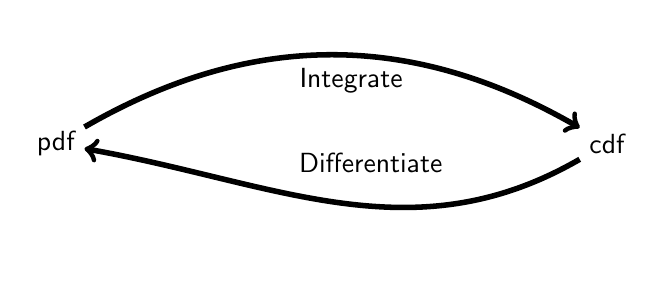
\begin{tikzpicture} 
\invisible<1-3>{\node (d1) at (-4, 3) [] {pdf};  } 
\invisible<1-5>{\node (f1) at (3, 3) [] {cdf} ; } 
\invisible<1-4>{\draw[->, line width=2pt] (d1) to [out=30, in=150] (f1) ; } 
\invisible<1-4>{\node (d2) at (-0.25, 3.8) [] {Integrate} ; } 

\invisible<1-6>{\node (f2) at (0, 2.75) [] {Differentiate} ; } 


\invisible<1-6>{\draw[->, line width=2pt] (f1) to [out=210, in=350] (d1); } 
\end{tikzpicture}
\end{center}
\pause \pause \pause \pause 



\end{frame}


\begin{frame}
\frametitle{Uniform Random Variable} 
 
 
 Suppose $X \sim Uniform(0,1)$, then \pause 
 \begin{eqnarray} 
\invisible<1>{ F(t) & = & P(X\leq t)  \nonumber } \pause \\
\invisible<1-2>{ & = & 0 \text{, if $t< 0$ } \nonumber } \pause \\
\invisible<1-3>{ & = & 1 \text{, if $t >1$ } \nonumber } \pause \\
\invisible<1-4>{ & = & t \text{, if $t \in [0,1]$ } \nonumber } 
 \end{eqnarray}



\scalebox{0.35}{\includegraphics{uniform1.pdf}}
\scalebox{0.35}{\includegraphics{cdfuniform.pdf}}
 
 
 \end{frame}

\begin{frame}
\frametitle{Expectation With Continuous Random Variables} 

\begin{defn} 
If $X$ is a continuous random variable then, 
\begin{eqnarray}
E[X] & = & \int_{-\infty}^{\infty} x f(x) dx \nonumber 
\end{eqnarray}
\end{defn} 


\end{frame}


\begin{frame}
Suppose $X \sim Uniform(0,1)$.  What is $E[X]$? \pause 
\begin{eqnarray}
\invisible<1>{E[X]} \pause\invisible<1-2>{ & = & \int_{-\infty}^{\infty} xf(x)dx \nonumber } \pause \\
\invisible<1-3>{& = & \int_{-\infty}^{0} x 0 dx + \int_{0}^{1} x 1 dx + \int_{1}^{\infty} x 0 dx \nonumber} \pause  \\
\invisible<1-4>{& = & 0 +  \frac{x^{2}}{2} |^{1}_{0} + 0 \nonumber } \pause \\
\invisible<1-5>{& = & 0 + \frac{1}{2} + 0 \nonumber } \pause \\
\invisible<1-6>{& = & \frac{1}{2} \nonumber } 
\end{eqnarray}


\end{frame}


\begin{frame}
\frametitle{Expectations of Functions} 
\begin{prop} 
Suppose $X$ is a continuous random variable and $g:\Re \rightarrow \Re$ (that isn't crazy).  Then, 
\begin{eqnarray}
E[g(X)] & = & \int_{-\infty}^{\infty} g(x)f(x)dx \nonumber 
\end{eqnarray}
\end{prop} 

\end{frame}


\begin{frame}
\frametitle{Expectations of Functions} 

Suppose $g(X) = X^2$  and $X \sim \text{Uniform}(0,1)$.  What is E[g(X)]? \pause 

\begin{eqnarray}
\invisible<1>{E[g(X)]} \pause \invisible<1-2>{ & = & \int_{-\infty}^{\infty} g(x)f(x)dx \nonumber} \pause  \\
\invisible<1-3>{& = & \int_{0}^{1} x^2dx \nonumber } \pause \\
\invisible<1-4>{& = & \frac{x^3}{3}|^{1}_{0} \nonumber } \pause \\
\invisible<1-5>{& = & \frac{1}{3} \nonumber}  
\end{eqnarray}


\end{frame}


\begin{frame}

\begin{cor} 
Suppose $X$ is a continuous random variable.  Then, 
\begin{eqnarray}
E[aX + b] & = & aE[X] + b\nonumber 
\end{eqnarray}
\end{cor}
\pause 

\begin{proof}
\begin{eqnarray}
\invisible<1>{E[aX + b] & = & \int_{-\infty}^{\infty} (a x + b)f(x) dx \nonumber \\} \pause 
\invisible<1-2>{& = & a \int_{-\infty}^{\infty} x f(x) dx + b \int_{-\infty}^{\infty} f(x)dx \nonumber \\} \pause 
\invisible<1-3>{& = & a E[X]  + b \times 1 \nonumber } 
\end{eqnarray}


\end{proof}


\end{frame}




\begin{frame}


\begin{defn} 
Variance.  If $X$ is a continuous random variable, define its variance, $Var(X)$, 
\begin{eqnarray}
Var(X) & = & E[(X- E[X])^2] \nonumber \\
& = & \int_{-\infty}^{\infty} (x - E[X])^2f(x) dx \nonumber \\
& = & E[X^2] - E[X]^2 \nonumber 
\end{eqnarray}
\end{defn}

\end{frame}



\begin{frame}
\frametitle{Variance: Random Variable} 

$X \sim \text{Uniform}(0,1)$.  What is $Var(X)$? \pause   

\begin{eqnarray} 
\invisible<1>{E[X^2] & = & \frac{1}{3} \nonumber } \pause \\
\invisible<1-2>{E[X]^2 & = & \left(\frac{1}{2}\right)^2 \nonumber } \pause \\
\invisible<1-3>{& = & \frac{1}{4} \nonumber} \pause  
\end{eqnarray}

\begin{eqnarray}
\invisible<1-4>{Var(X) & =& E[X^2] - E[X]^2 } \pause \nonumber \\
\invisible<1-5>{ & = &  \frac{1}{3} - \frac{1}{4} = \alert{\frac{1}{12}}} \nonumber 
\end{eqnarray}

\end{frame}



\begin{frame}
\frametitle{Famous Continuous Distributions}

\begin{itemize}
\item[-] Normal Distribution
\item[-] Gamma distribution 
\item[-] $\chi^{2}$ Distribution
\item[-] $t$ Distribution
\item[-] Beta, Dirichlet distributions (not today!)
\item[-] $F$-distribution (not today!)
\end{itemize}



\end{frame}


\begin{frame}

\begin{defn}
Suppose $X$ is a random variable with $X \in \Re$ and \alert{density}

\begin{eqnarray}
f(x) & = & \frac{1}{\sqrt{2\pi \sigma^2}}\exp\left(-\frac{(x - \mu)^2}{2\sigma^2}\right) \nonumber 
\end{eqnarray}

Then $X$ is a \alert{normally} distributed random variable with parameters $\mu$ and $\sigma^2$.  \\


Equivalently, we'll write 
\begin{eqnarray}
X & \sim & \text{Normal}(\mu, \sigma^2) \nonumber 
\end{eqnarray}




\end{defn}
\end{frame}

\begin{frame}
\frametitle{Support for President Obama} 

Suppose we are interested in modeling \alert{presidential approval} \pause 
\begin{itemize}
\invisible<1>{\item[-] Let $Y$ represent random variable: proportion of population who ``approves job president is doing"} \pause 
\invisible<1-2>{\item[-] Individual responses (that constitute proportion) are \alert{independent} and \alert{identically} distributed (sufficient, not necessary) and we take the average of those individual responses} \pause 
\invisible<1-3>{\item[-] Observe \alert{many} responses ($N\rightarrow \infty$)} \pause 
\invisible<1-4>{\item[-] Then (by Central Limit Theorm) $Y$ is \alert{Normally} distributed, or } \pause 
\end{itemize}
\begin{eqnarray}
\invisible<1-5>{Y& \sim & \text{Normal}(\mu, \sigma^2) \nonumber } \pause \\
\invisible<1-6>{f(y) & = & \frac{\exp\left(-\frac{(y-\mu)^2}{2\sigma^2} \right)}{\sqrt{2\pi \sigma^2}} \nonumber } 
%\text{Mean} & = & \alert{\mu} \nonumber \\
%\text{Variance} & = & \alert{\sigma^2} \nonumber  
\end{eqnarray}

\end{frame}


\begin{frame}
\frametitle{Central Limit Theorem}
We'll prove it on Thursday. \\
Simulation: 
\only<1>{\scalebox{0.5}{\includegraphics{CLT2.pdf}}}\only<2>{\scalebox{0.5}{\includegraphics{CLT3.pdf}}}\only<3>{\scalebox{0.5}{\includegraphics{CLT4.pdf}}}\only<4>{\scalebox{0.5}{\includegraphics{CLT5.pdf}}}\only<5>{\scalebox{0.5}{\includegraphics{CLT6.pdf}}}\only<6>{\scalebox{0.5}{\includegraphics{CLT7.pdf}}}\only<7>{\scalebox{0.5}{\includegraphics{CLT8.pdf}}}\only<8>{\scalebox{0.5}{\includegraphics{CLT9.pdf}}}\only<9>{\scalebox{0.5}{\includegraphics{CLT10.pdf}}}\only<10>{\scalebox{0.5}{\includegraphics{CLT11.pdf}}}\only<11>{\scalebox{0.5}{\includegraphics{CLT12.pdf}}}\only<12>{\scalebox{0.5}{\includegraphics{CLT13.pdf}}}\only<13>{\scalebox{0.5}{\includegraphics{CLT14.pdf}}}\only<14>{\scalebox{0.5}{\includegraphics{CLT15.pdf}}}\only<15>{\scalebox{0.5}{\includegraphics{CLT16.pdf}}}\only<16>{\scalebox{0.5}{\includegraphics{CLT17.pdf}}}\only<17>{\scalebox{0.5}{\includegraphics{CLT18.pdf}}}\only<18>{\scalebox{0.5}{\includegraphics{CLT19.pdf}}}\only<19>{\scalebox{0.5}{\includegraphics{CLT20.pdf}}}\only<20>{\scalebox{0.5}{\includegraphics{CLT21.pdf}}}\only<21>{\scalebox{0.5}{\includegraphics{CLT22.pdf}}}\only<22>{\scalebox{0.5}{\includegraphics{CLT23.pdf}}}\only<23>{\scalebox{0.5}{\includegraphics{CLT24.pdf}}}\only<24>{\scalebox{0.5}{\includegraphics{CLT25.pdf}}}\only<25>{\scalebox{0.5}{\includegraphics{CLT26.pdf}}}\only<26>{\scalebox{0.5}{\includegraphics{CLT27.pdf}}}\only<27>{\scalebox{0.5}{\includegraphics{CLT28.pdf}}}\only<28>{\scalebox{0.5}{\includegraphics{CLT29.pdf}}}\only<29>{\scalebox{0.5}{\includegraphics{CLT30.pdf}}}\only<30>{\scalebox{0.5}{\includegraphics{CLT31.pdf}}}\only<31>{\scalebox{0.5}{\includegraphics{CLT32.pdf}}}\only<32>{\scalebox{0.5}{\includegraphics{CLT33.pdf}}}\only<33>{\scalebox{0.5}{\includegraphics{CLT34.pdf}}}\only<34>{\scalebox{0.5}{\includegraphics{CLT35.pdf}}}\only<35>{\scalebox{0.5}{\includegraphics{CLT36.pdf}}}\only<36>{\scalebox{0.5}{\includegraphics{CLT37.pdf}}}\only<37>{\scalebox{0.5}{\includegraphics{CLT38.pdf}}}\only<38>{\scalebox{0.5}{\includegraphics{CLT39.pdf}}}\only<39>{\scalebox{0.5}{\includegraphics{CLT40.pdf}}}\only<40>{\scalebox{0.5}{\includegraphics{CLT41.pdf}}}\only<41>{\scalebox{0.5}{\includegraphics{CLT42.pdf}}}\only<42>{\scalebox{0.5}{\includegraphics{CLT43.pdf}}}\only<43>{\scalebox{0.5}{\includegraphics{CLT44.pdf}}}\only<44>{\scalebox{0.5}{\includegraphics{CLT45.pdf}}}\only<45>{\scalebox{0.5}{\includegraphics{CLT46.pdf}}}\only<46>{\scalebox{0.5}{\includegraphics{CLT47.pdf}}}\only<47>{\scalebox{0.5}{\includegraphics{CLT48.pdf}}}\only<48>{\scalebox{0.5}{\includegraphics{CLT49.pdf}}}\only<49>{\scalebox{0.5}{\includegraphics{CLT50.pdf}}} 



\end{frame}






\begin{frame}
\frametitle{Expected Value/Variance of Normal Distribution}

$Z$ is a standard normal distribution if \pause 
\invisible<1>{\begin{eqnarray}
Z & \sim & \text{Normal}(0,1) \nonumber 
\end{eqnarray}
} \pause 



\invisible<1-2>{We'll call the cumulative distribution function of $Z$, } \pause 
\begin{eqnarray}
\invisible<1-3>{F_{Z}(x) & = & \frac{1}{\sqrt{2\pi} }\int_{-\infty}^{x} \exp(-z^2/2) dz \nonumber } \pause 
\end{eqnarray}

\invisible<1-4>{
\begin{prop} 
\alert{Scale/Location}.  If $Z \sim N(0,1)$, then $X = aZ + b$ is, 
\begin{eqnarray}
X & \sim & \text{Normal} (b, a^2) \nonumber 
\end{eqnarray}
\end{prop}

}

\end{frame}




\begin{frame}
\frametitle{Intuition}

Suppose $Z \sim \text{Normal}(0,1)$.  \\
\invisible<1>{$Y = 2Z + 6$} \\
\invisible<1-2>{$Y \sim \text{Normal}(6, 4)$} 

\begin{center}
\only<1-2>{\scalebox{0.6}{\includegraphics{Normal1.pdf}}}
\only<3->{\scalebox{0.6}{\includegraphics{Normal2.pdf}}}
\end{center}
\pause \pause 

\end{frame}



\begin{frame}
\frametitle{Proof:$Z \sim N(0,1)$ and $Y = aZ + b$, then  $Y \sim N(b, a^2)$ } 
To prove\pause \invisible<1>{ we need to show that density for $Y$ is a normal distribution. } \pause  \\
\invisible<1-2>{That is, we'll show $F_{Y}(x)$ is Normal cdf.} \pause   \\
\invisible<1-3>{Call $F_{Z}(x)$ cdf for standardized normal.} \pause   

\begin{eqnarray}
\invisible<1-4>{F_{Y} (x) & = & P(Y \leq x) \nonumber } \pause  \\
\invisible<1-5>{& = & P(aZ + b \leq x) \nonumber } \pause  \\
\invisible<1-6>{& = & P(Z \leq \left[\frac{x - b}{a} \right] ) \nonumber } \pause  \\
\invisible<1-7>{& = & \frac{1}{\sqrt{2\pi} } \int_{-\infty}^{\frac{x-b}{a} } \exp( - \frac{z^2}{2} ) dz \nonumber} \pause  \\
\invisible<1-8>{ & = &F_{Z} (\frac{x - b}{a} )\nonumber }
 \end{eqnarray}








\end{frame}

\begin{frame}
\frametitle{Proof:$Z \sim N(0,1)$ and $Y = aZ + b$, then  $Y \sim N(b, a^2)$ } 

So, we can work with $F_{Z}(\frac{x - b}{a} )$.  \pause 
\begin{eqnarray}
\invisible<1>{\frac{\partial F_{Y}(x) }{\partial x} & =& \frac{\partial F_{Z} (\frac{x - b}{a} ) }{\partial x} \nonumber } \pause \\
\invisible<1-2>{& = & f_{Z} (\frac{x - b}{a} ) \frac{1}{a}  \text{ By the chain rule }} \pause \nonumber \\
\invisible<1-3>{& = & \frac{1}{\sqrt{2 \pi } a } \exp\left[-\frac{\left(\frac{x-b}{a} \right)^2}{2 }\right] \nonumber \text{ By definition of $f_{Z}(x)$ or FTC}} \pause \\
\invisible<1-4>{& = & \frac{1}{\sqrt{2 \pi } a } \exp\left[-\frac{\left(x-b\right)^2}{2a^2 }\right] \nonumber } \pause \\
\invisible<1-5>{& = & \text{Normal} (b, a^2) \nonumber }
\end{eqnarray}

\end{frame}

\begin{frame}
\frametitle{Expectation and Variance}

Assume we know: 
\begin{eqnarray}
E[Z]  & = & 0 \nonumber \\
Var(Z) & = & 1 \nonumber 
\end{eqnarray}
\pause 
\invisible<1>{This implies that, for $Y \sim \text{Normal}(\mu, \sigma^2)$} \pause 
\begin{eqnarray} 
\invisible<1-2>{E[Y] & = & E[\sigma Z + \mu] \nonumber } \pause \\
\invisible<1-3>{& = & \sigma E[Z] + \mu \nonumber } \pause \\
\invisible<1-4>{& = & \mu \nonumber } \pause \\
\invisible<1-5>{Var(Y) & = & Var(\sigma Z + \mu) \nonumber } \pause \\
\invisible<1-6>{ & = & \sigma^2 Var(Z) + Var(\mu) \nonumber } \pause \\
\invisible<1-7>{ & = & \sigma^2 + 0 \nonumber } \pause \\
\invisible<1-8>{ & =& \sigma^2 \nonumber } 
\end{eqnarray}

\end{frame}





\begin{frame}
\frametitle{Back To Obama} 

Suppose $\mu = 0.39$ and $\sigma^2 = 0.0025$ \pause  \\
\invisible<1>{$P(Y\geq 0.45)$ (What is the probability it isn't that bad?) ? } \pause 
\begin{eqnarray} 
\invisible<1-2>{P(Y \geq 0.45)  &  = & 1 - P(Y \leq 0.45 ) \nonumber} \pause  \\
\invisible<1-3>{& = &  1 - P(0.05 Z + 0.39 \leq  0.45)   \nonumber } \pause\\
\invisible<1-4>{& = & 1 - P(Z \leq \frac{0.45-0.39 }{0.05} ) \nonumber} \pause \\
\invisible<1-5>{& = & 1 - \frac{1}{\sqrt{2\pi} } \int_{-\infty}^{6/5} \exp(-z^2/2) dz } \pause   \nonumber \\
\invisible<1-6>{& = & 1 - F_{Z} (\frac{6}{5} ) \nonumber } \pause\\
\invisible<1-7>{& = & 0.1150697 \nonumber } 
\end{eqnarray}


\end{frame}


\begin{frame}
\frametitle{Back To Obama } 

Via simulation: \\

$<$ code $>$

{\tt \hspace{0.025in} draws<- rnorm(1e7, mean = 0.39, sd = sqrt(0.0025) ) \\
\hspace{0.025in} greater<- which(draws>0.45) \\
\hspace{0.025in} p.45 <- length(greater)/1e7 \\
\hspace{0.025in} print(p.45) \\
\hspace{0.025in} [1] 0.1149824
}


$</$ code $>$
\end{frame}

\begin{frame}
\frametitle{The Gamma Function}

\begin{defn}
Suppose $\alpha>0$.  Then define $\Gamma(\alpha)$ as 
\begin{eqnarray}
\Gamma(\alpha) & = & \int_{0}^{\infty} y^{\alpha- 1} e^{-y} dy \nonumber 
\end{eqnarray}
\end{defn}

\begin{itemize}
\item[-] For $\alpha \in \{1, 2, 3, \hdots\}$\\
 $\Gamma(\alpha) = (\alpha- 1)!$
\item[-] $\Gamma(\frac{1}{2}) = \sqrt{\pi}$
\end{itemize}


\end{frame}


\begin{frame}
\frametitle{Gamma Distribution}

Suppose we have $\Gamma(\alpha)$,  \pause 
\begin{eqnarray}
\invisible<1>{\frac{\Gamma(\alpha)}{\Gamma(\alpha)} & = & \frac{\int_{0}^{\infty} y^{\alpha-1} e^{-y} dy}{\Gamma(\alpha)} \nonumber \\
1 & = & \int_{0}^{\infty} \frac{1}{\Gamma(\alpha)} y^{\alpha-1} e^{-y} dy \nonumber } \pause 
\end{eqnarray}

\invisible<1-2>{Set $X = Y/\beta$} \pause 

\begin{eqnarray}
\invisible<1-3>{F(x) = P(X \leq x) & = & P(Y/\beta \leq x ) \nonumber \\} 
\invisible<1-4>{& = & P(Y \leq x \beta ) \nonumber \\} 
 \invisible<1-5>{& = & F_{Y} (x \beta) \nonumber\\} 
  \invisible<1-6>{\frac{\partial F_{Y} (x \beta) }{\partial x} & = & f_{Y} (x \beta) \beta \nonumber } 
\end{eqnarray}
 \pause \pause \pause \pause 
 \invisible<1-7>{The result is:} \pause 
 \begin{eqnarray}
\invisible<1-8>{f(x|\alpha, \beta) & = & \frac{\beta^{\alpha}}{\Gamma(\alpha)} x^{\alpha - 1} e^{-x\beta}  \nonumber }
 \end{eqnarray}



\end{frame}


\begin{frame}

\begin{defn}
Suppose $X$ is a continuous random variable, with $X \geq 0$.  Then if the pdf of $X$ is 
 \begin{eqnarray}
f(x|\alpha, \beta) & = & \frac{\beta^{\alpha}}{\Gamma(\alpha)} x^{\alpha - 1} e^{-x\beta}  \nonumber 
 \end{eqnarray}

if $x\geq 0$ and $0$ otherwise, we will say $X$ is a Gamma distribution. 
\begin{eqnarray}
X & \sim & \text{Gamma}(\alpha, \beta) \nonumber 
\end{eqnarray}

\end{defn}


\end{frame}


\begin{frame}
\frametitle{Gamma Distribution}

Suppose $X \sim \text{Gamma}(\alpha, \beta)$ \pause 
\begin{eqnarray}
\invisible<1>{E[X] & = & \frac{\alpha}{\beta} \nonumber \\}
\invisible<1-2>{\text{var}(X) & = & \frac{\alpha}{\beta^2} \nonumber }
\end{eqnarray}

\pause \pause 

\invisible<1-3>{Suppose $\alpha = 1$ and $\beta = \lambda$.  If } 
\begin{eqnarray}
\invisible<1-4>{X & \sim & \text{Gamma}(1, \lambda) \nonumber \\}
\invisible<1-5>{f(x|1, \lambda ) & = & \lambda e^{- x \lambda}  \nonumber}
\end{eqnarray}

\pause \pause \pause 

\invisible<1-6>{We will say } \pause 
\begin{eqnarray}
\invisible<1-7>{X & \sim & \text{Exponential}(\lambda) \nonumber }
\end{eqnarray}


\end{frame}

\begin{frame}
\frametitle{Properties of Gamma Distributions}

\begin{prop}
Suppose we have a sequence of independent random variables, with 
\begin{eqnarray}
X_{i} & \sim & \text{Gamma}(\alpha_{i}, \beta) \nonumber 
\end{eqnarray}
Then 
\begin{eqnarray}
Y = \sum_{i=1}^{N} X_{i} \nonumber 
\end{eqnarray}

$Y \sim \text{Gamma}(\sum_{i=1}^{N} \alpha_{i} , \beta) $


\end{prop}


\end{frame}





\begin{frame}
We can evaluate in {\tt R} with {\tt dgamma} and simulate with {\tt rgamma}\\

$X \sim \text{Gamma}(3, 5)$ and we evaluate at 3, \\
{\tt dgamma(3, shape= 3, rate = 5)}\\
and we can simulate with \\
{\tt rgamma(1000, shape = 3, rate = 5)} 




\end{frame}


\begin{frame}

\begin{center}

\scalebox{0.6}{\includegraphics{GammaPlot.pdf}}

\end{center}

\end{frame}


\begin{frame}
\frametitle{$\chi^{2}$ Distribution}

Suppose $Z \sim \text{Normal}(0,1)$. \pause   \\
\invisible<1>{Consider $X = Z^2$} \pause 
\begin{eqnarray}
\invisible<1-2>{F_{X}(x)   & = &  P(X \leq x) \nonumber \\ } \pause 
\invisible<1-3>{& = & P(Z^2 \leq x ) \nonumber \\} \pause 
 \invisible<1-4>{& = & P(-\sqrt{x} \leq Z \leq \sqrt{x}) \nonumber \\} \pause 
 \invisible<1-5>{& = & \frac{1}{\sqrt{2\pi}} \int_{-\sqrt{x}}^{\sqrt{x} } e^{-\frac{z^2}{2}} dz \nonumber \\} \pause 
 \invisible<1-6>{& = & F_{Z} (\sqrt{x}) - F_{Z} (-\sqrt{x}) \nonumber } 
\end{eqnarray}
\invisible<1-7>{The pdf then is } \pause 

\begin{eqnarray}
\invisible<1-8>{\frac{\partial F_{X}(x) }{\partial x }  & = & f_{Z} (\sqrt{x}) \frac{1}{2\sqrt{x}} + f_{Z}(-\sqrt{x}) \frac{1}{2\sqrt{x}} \nonumber } 
\end{eqnarray}

\pause 




\end{frame}

\begin{frame}
\frametitle{$\chi^2$ Distribution}
\begin{eqnarray}
\frac{\partial F_{X}(x) }{\partial x }  & = & f_{Z} (\sqrt{x}) \frac{1}{2\sqrt{x}} + f_{Z}(-\sqrt{x}) \frac{1}{2\sqrt{x}} \nonumber \pause \\
\invisible<1>{& = & \frac{1}{\sqrt{x}}\frac{1}{2 \sqrt{2\pi}} ( 2e^{-\frac{x}{2}}) \nonumber \\} \pause 
\invisible<1-2>{& = & \frac{1}{\sqrt{x}}\frac{1}{\sqrt{2\pi}} ( e^{-\frac{x}{2}}) \nonumber \\} \pause 
\invisible<1-3>{& = & \frac{(\frac{1}{2})^{1/2}}{\Gamma(\frac{1}{2})}\left(x^{1/2 - 1} e^{-\frac{x}{2}}\right) \nonumber } \pause 
\end{eqnarray}

\invisible<1-4>{$X \sim \text{Gamma}(1/2, 1/2)$} \pause 

\invisible<1-5>{Then if $X = \sum_{i=1}^{N} Z^2$\\} \pause 

\invisible<1-6>{$X \sim \text{Gamma}(n/2, 1/2) $}



\end{frame}


\begin{frame}

\begin{defn}
Suppose $X$ is a continuous random variable with $X\geq 0$, with pdf 

\begin{eqnarray}
f(x) & = & \frac{1}{2^{n/2} \Gamma(n/2) } x^{n/2 - 1} e^{-x/2} \nonumber 
\end{eqnarray}

Then we will say $X$ is a $\chi^2$ distribution with $n$ degrees of freedom.  Equivalently,

\begin{eqnarray}
X & \sim & \chi^{2}(n) \nonumber 
\end{eqnarray}

\end{defn}



\end{frame}


\begin{frame}

\only<1>{\scalebox{0.5}{\includegraphics{ChiSq1.pdf}}}
\only<2>{\scalebox{0.5}{\includegraphics{ChiSq2.pdf}}}
\only<3>{\scalebox{0.5}{\includegraphics{ChiSq3.pdf}}}
\only<4>{\scalebox{0.5}{\includegraphics{ChiSq4.pdf}}}
\only<5>{\scalebox{0.5}{\includegraphics{ChiSq5.pdf}}}
\only<6>{\scalebox{0.5}{\includegraphics{ChiSq6.pdf}}}
\only<7>{\scalebox{0.5}{\includegraphics{ChiSq7.pdf}}}
\only<8>{\scalebox{0.5}{\includegraphics{ChiSq8.pdf}}}
\only<9>{\scalebox{0.5}{\includegraphics{ChiSq9.pdf}}}
\only<10>{\scalebox{0.5}{\includegraphics{ChiSq10.pdf}}}


\end{frame}


\begin{frame}
\frametitle{$\chi^2$ Properties}

Suppose $X \sim \chi^2(n)$
\begin{eqnarray}
E[X] & = & E\left[\sum_{i=1}^{N} Z_{i}^2\right] \nonumber \\
 & = & \sum_{i=1}^{N} E[Z_{i}^{2} ] \nonumber \\
\text{var}(Z_{i} ) & = & E[Z_{i}^2] - E[Z_{i}]^2 \nonumber\\
1 & = & E[Z_{i}^2]- 0 \nonumber \\
E[X] & = & n \nonumber 
 \end{eqnarray}



\end{frame}

\begin{frame}
\frametitle{$\chi^2$ Properties}

\begin{eqnarray}
\text{var}(X) & = & \sum_{i=1}^{N} \text{var}(Z_{i}^2) \nonumber \\
& = & \sum_{i=1}^{N} \left(E[Z_{i}^{4} ] - E[Z_{i}]^{2}  \right) \nonumber \\
& = & \sum_{i=1}^{N} \left(3 - 1\right ) = 2n \nonumber 
\end{eqnarray}

We will use the $\chi^2$ across statistics.  


\end{frame}


\begin{frame}
\frametitle{Student's $t$-Distribution}

\begin{defn}
Suppose $Z \sim \text{Normal}(0, 1)$ and $U \sim \chi^2(n)$.  Define the random variable $Y$ as, 

\begin{eqnarray}
Y & = & \frac{Z}{\sqrt{\frac{U}{n}}} \nonumber 
\end{eqnarray}

If $Z$ and $U$ are independent then $Y \sim t(n)$, with pdf 

\begin{eqnarray}
f(x) & = & \frac{\Gamma(\frac{n+1}{2})}{\sqrt{\pi n } \Gamma(\frac{n}{2})}\left(1 + \frac{x^2}{n}\right)^{-\frac{n+1}{2}} \nonumber 
\end{eqnarray}

We will use the t-distribution extensively for \alert{test-statistics}


\end{defn}



\end{frame}


\begin{frame}

\only<1>{\scalebox{0.5}{\includegraphics{tdist1.pdf}}}
\only<2>{\scalebox{0.5}{\includegraphics{tdist2.pdf}}}
\only<3>{\scalebox{0.5}{\includegraphics{tdist3.pdf}}}
\only<4>{\scalebox{0.5}{\includegraphics{tdist4.pdf}}}
\only<5>{\scalebox{0.5}{\includegraphics{tdist5.pdf}}}
\only<6>{\scalebox{0.5}{\includegraphics{tdist6.pdf}}}
\only<7>{\scalebox{0.5}{\includegraphics{tdist7.pdf}}}
\only<8>{\scalebox{0.5}{\includegraphics{tdist8.pdf}}}
\only<9>{\scalebox{0.5}{\includegraphics{tdist9.pdf}}}
\only<10>{\scalebox{0.5}{\includegraphics{tdist10.pdf}}}
\only<11>{\scalebox{0.5}{\includegraphics{tdist11.pdf}}}
\only<12>{\scalebox{0.5}{\includegraphics{tdist12.pdf}}}
\only<13>{\scalebox{0.5}{\includegraphics{tdist13.pdf}}}
\only<14>{\scalebox{0.5}{\includegraphics{tdist14.pdf}}}
\only<15>{\scalebox{0.5}{\includegraphics{tdist15.pdf}}}
\only<16>{\scalebox{0.5}{\includegraphics{tdist16.pdf}}}
\only<17>{\scalebox{0.5}{\includegraphics{tdist17.pdf}}}
\only<18>{\scalebox{0.5}{\includegraphics{tdist18.pdf}}}
\only<19>{\scalebox{0.5}{\includegraphics{tdist19.pdf}}}
\only<20>{\scalebox{0.5}{\includegraphics{tdist20.pdf}}}
\only<21>{\scalebox{0.5}{\includegraphics{tdist21.pdf}}}
\only<22>{\scalebox{0.5}{\includegraphics{tdist22.pdf}}}
\only<23>{\scalebox{0.5}{\includegraphics{tdist23.pdf}}}
\only<24>{\scalebox{0.5}{\includegraphics{tdist24.pdf}}}
\only<25>{\scalebox{0.5}{\includegraphics{tdist25.pdf}}}
\only<26>{\scalebox{0.5}{\includegraphics{tdist26.pdf}}}
\only<27>{\scalebox{0.5}{\includegraphics{tdist27.pdf}}}
\only<28>{\scalebox{0.5}{\includegraphics{tdist28.pdf}}}
\only<29>{\scalebox{0.5}{\includegraphics{tdist29.pdf}}}
\only<30>{\scalebox{0.5}{\includegraphics{tdist30.pdf}}}

\end{frame}






\begin{frame}
\frametitle{Student's $t$-Distribution, Properties}

Suppose $n = 1$, \alert{Cauchy} distribution

\only<1>{\scalebox{0.5}{\includegraphics{Cauchy1.pdf}}} 
\only<2->{
If $X \sim \text{Cauchy}(1)$, then:\\
$E[X] =$ undefined \\
var$(X)$ = undefined \\

If $X \sim t(2)$ \\
E[X] = 0  \\
$\text{var}(X) $ = undefined

}




\end{frame}


\begin{frame}
\frametitle{Student's $t$-Distribution, Properties}

Suppose $n>2$, then \\
$var(X) = \frac{n}{n-2}$ \\
As $n \rightarrow \infty$ var$(X) \rightarrow 1$.  



\end{frame}


\begin{frame}

Tomorrow: Joint Distributions and Multivariate Normal Distribution

\end{frame}






\end{document}
